\section{Financial Modelling}

\subsection{Brownian Motion}
\begin{definition}[Brownian Motion]
    A stochastic process $(B_t)_{t\ge0}$ is called a Brownian motion if it satisfies the following properties:
    \begin{itemize}
        \item \textbf{Starts at 0} : $B_0 = 0$ (almost surely).
        \item \textbf{Continuous sample path} : $t\to B_t$ is continuous (almost surely).
        \item \textbf{Independence of increments} : For any finite sequence of time $t_0<t_1<\dots<t_n$, the increments
        \begin{align*}
            B_{t_1} - B_{t_0}, B_{t_2} - B_{t_1}, \dots, B_{t_n} - B_{t_{n-1}}
        \end{align*}
        are independent.
        \item For all $0\le s < t$, $B_t - B_s \sim \mathcal{N}(0, t-s)$.
    \end{itemize}
\end{definition}

\noindent\newline \textbf{Remark} : Brownian motion can be seen under the lens of Random Walk when we scale the interval between steps of the walk down infinitesimally.

\subsection{Geometric Brownian Motion}
\begin{definition}[Market Return] 
    Two definitions of market returns:
    \begin{itemize}
        \item Standard return is defined as:
        \begin{align*}
            \frac{\Delta S_t}{S_t} = \frac{S_{t+\Delta t} - S_t}{S_t}
        \end{align*}

        \item Log return is defined (for $t\ge 0$) as:
        \begin{align*}
            \Delta \log S_t = \log S_{t+\Delta t} - \log S_t = \log\frac{S_{t+\Delta t}}{S_t} = \log\Bigg( 1 + \frac{\Delta S_t}{S_t}\Bigg)
        \end{align*}
    \end{itemize}

    \noindent Where $S_t$ is the market price at time $t\ge0$.
\end{definition}

\begin{proposition}{Geometric Brownian Motion}{geom_brownian_motion}
    The Geometric Brownian Motion $(S_t)_{t\ge 0}$ is a stochastic process, which is the solution to the Stochastic Differential Equation of the form
    \begin{align*}
        dS_t = \mu S_t dt + \sigma S_t dB_t
    \end{align*}

    \noindent The solution for the above equation is given by:
    \begin{align*}
        \boxed{
        S_t = S_0 \exp\Bigg( \sigma B_t + \Bigg( \mu - \frac{\sigma^2}{2} \Bigg)t \Bigg), t \ge 0
        }
    \end{align*}
\end{proposition}

\begin{proof*}[Proposition \ref{prop:geom_brownian_motion}]
    The asset prices $(S_t)_{t\ge0}$ satisfies:
    \begin{align}
        \frac{dS_t}{S_t} = \frac{S_{t+dt} - S_t}{S_t} = \mu dt + \sigma dB_t
    \end{align}

    \noindent Taking the differential of the logarithm of asset price, we have:
    \begin{align*}
        d\log S_t &\approx \log S_{t+dt} - \log S_t \\
            &= \log\frac{S_{t+dt}}{S_t} \\
            &= \log \biggRound{
                1 + \frac{dS_t}{S_t}
            } \\
            &= \log \bigRound{ 1 + \mu dt + \sigma dB_t } \\
            &\approx \mu dt + \sigma dB_t - \frac{(\mu dt + \sigma dB_t)^2}{2} \ \ \ \biggRound{\log(x+1) \to x - \frac{x^2}{2} \text{ as } x \to 0} \\
            &\approx \mu dt + \sigma dB_t - \frac{\mu^2}{2}(dt)^2 - \mu\sigma dtdB_t - \frac{\sigma^2}{2}(dB_t)^2 \\
            &= \mu dt + \sigma dB_t - \frac{\sigma^2}{2}dt \\
        \implies
        \log S_t &= \log S_0 + \sigma dB_t + \biggRound{
            \mu - \frac{\sigma^2}{2}
        }t
    \end{align*}

    \noindent From the above, we derive the solution to the SDE $dS_t = \mu S_tdt + \sigma S_t dB_t$:
    \begin{align}
        S_t = S_0 \exp\biggRound{
            \sigma B_t + \biggRound{\mu - \frac{\sigma^2}{2}}t
        }, \ \ \ t \ge 0
    \end{align}
\end{proof*}


\begin{proposition}{Distribution of Geometric BM}{dist_of_gbm}
    At any time $T > 0$, the random variable 
    \begin{align*}
        S_T = S_0 \exp\Bigg( \sigma B_T + \Bigg( \mu - \frac{\sigma^2}{2} \Bigg)T \Bigg)
    \end{align*}
    \noindent has the \textbf{log-normal distribution} with the density function:
    \begin{align*}
        \boxed{
            f_{S_T}(x) = \frac{1}{\sigma x \sqrt{2\pi T}}\exp\Bigg( 
                -\frac{1}{2\sigma^2 T} \Bigg(\log x - \log S_0 - \Bigg( \mu - \frac{\sigma^2}{2} \Bigg)T \Bigg)^2
            \Bigg)
        }
    \end{align*}
\end{proposition}

\begin{proof*}[Proposition \ref{prop:dist_of_gbm}]
    For any $x\in\R$, we have:
    \begin{align*}
        P(S_t \le x) &= P\biggRound{
            S_0 \exp\biggRound{
                \sigma B_t + \biggRound{\mu - \frac{\sigma^2}{2}}t
            } \le x
        } \\
        &= P\biggRound{
            \log S_0 + \sigma B_t + \biggRound{ \mu - \frac{\sigma^2}{2} }t  \le \log x
        } = P\biggRound{
            \sigma B_t + \biggRound{ \mu - \frac{\sigma^2}{2} }t \le \log \frac{x}{S_0}
        }\\
        &= P\biggRound{
            B_t \le \frac{1}{\sigma} \biggSquare{
                \log\frac{x}{S_0} - \biggRound{ \mu - \frac{\sigma^2}{2} }t
            }
        }
    \end{align*}

    \noindent We have:
    \begin{align*}
        B_t \sim \mathcal{N}(0,t) \implies B_t = Z\sqrt{t}, \ \ \ (Z\sim \mathcal{N}(0,1))
    \end{align*}

    \noindent Hence, we have:
    \begin{align*}
        P(S_t \le x) 
            &= P\biggRound{
                    Z \le \frac{1}{\sigma\sqrt{t}} \biggSquare{
                    \log\frac{x}{S_0} - \biggRound{ \mu - \frac{\sigma^2}{2} }t
                }
            } \\
            &= \Phi \biggRound{
                \frac{1}{\sigma\sqrt{t}} \biggSquare{
                    \log\frac{x}{S_0} - \biggRound{ \mu - \frac{\sigma^2}{2} }t
                }
            } = \Phi \biggRound{
                \frac{1}{\sigma\sqrt{t}} \biggSquare{
                    \log x - \log S_0 - \biggRound{ \mu - \frac{\sigma^2}{2} }t
                }
            }
    \end{align*}

    \noindent The above CDF is of a random variable from the distribution $Lognormal({\bf M, S})$ where:
    \begin{align*}
        {\bf M} &= \log S_0 + \biggRound{ \mu - \frac{\sigma^2}{2} }t \\
        {\bf S} &= t\sigma^2
    \end{align*}
\end{proof*}

\subsection{Distribution of market return}
\textbf{Overview} : Even though we can model the market returns using Brownian Motion and Geometric Brownian Motion, the assumption of Gaussian market returns is often not true. We can use the following visualizations/tests to verify that assumption:
\begin{itemize}
    \item Empirical vs. estimated Gaussian CDFs.
    \item QQ plot.
    \item The one-sample Kolmogorov-Smirnov test.
\end{itemize}

\noindent\newline For example, the following visualization illustrates how the Gaussian return assumption can under-estimate extreme events.
\begin{figure}[ht]
    \centering
    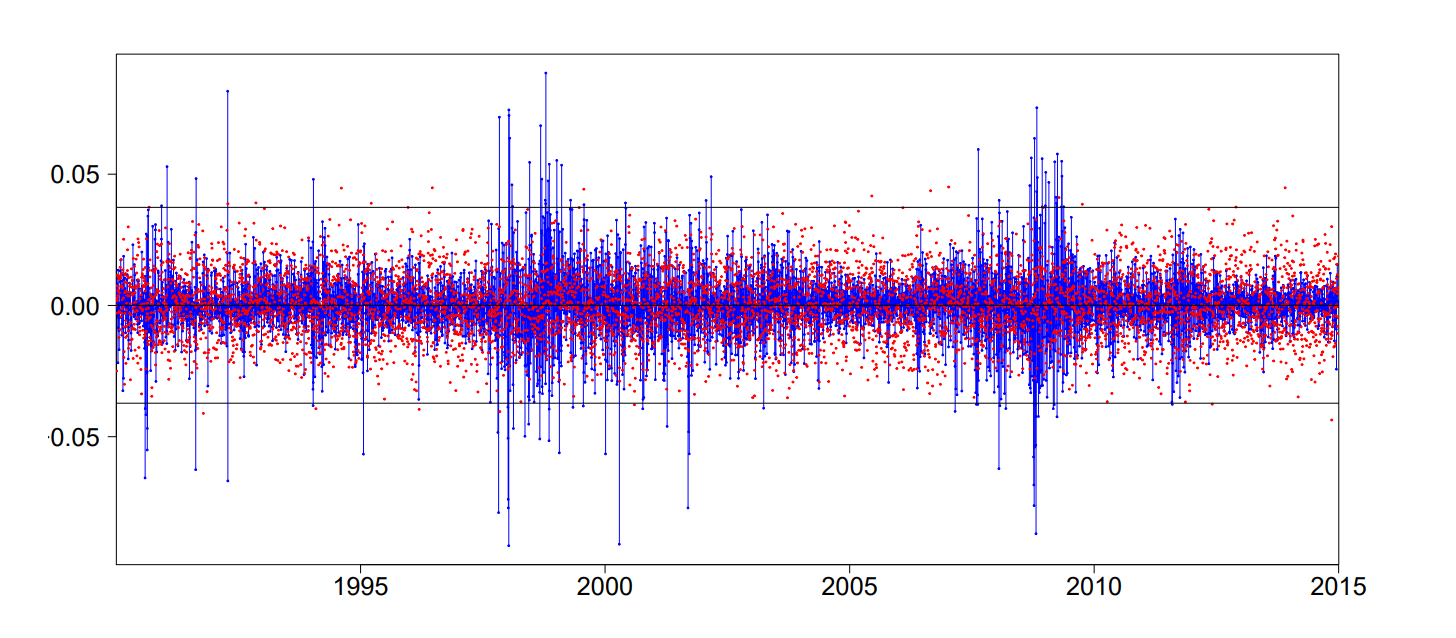
\includegraphics[width=\textwidth]{figures/emprical-vs-gaussian-cdf.png}
    \caption{Market returns (blue) vs normalized Gaussian returns (red) (figure sampled from \cite{book:privault})}
    \label{fig:empirical-vs-gaussian-cdfs}
\end{figure}

\noindent \newline In later section, we will see that in order to alleviate this problem, \textbf{Gram-Charlier expansion} is proposed for higher-order estimate of the empirical CDF of market returns.

\begin{definition}[Cumulants]
    The cumulants of a random variable $X$ is essentially an alternative to moments. The cumulants are derived from the \textbf{cumulant generating function}:
    \begin{align*}
        K_X(t) &= \log M_X(t) = \log \mathbb{E}[e^{tX}] \\
        \kappa_n^X &= K_X^{(n)}(0) \ \ \ (n^{th} \text{ order cumulant})
    \end{align*}
\end{definition}

\textbf{Remark} : We have the following remarks about the cumulant:
\begin{itemize}
    \item $\kappa_1^X=\mathbb{E}[X]$ (Mean).
    \item $\kappa_2^X=Var(X)=\mathbb{E}\Big[ (X - \mu_X)^2 \Big]$ (Variance).
    \item $\kappa_3^X=\mathbb{E}\Big[ (X - \mu_X)^3 \Big]$ (Third central moment).
    \item $\kappa_4^X=\mathbb{E}\Big[ (X - \mu_X)^4 \Big] - 3(\kappa_2^X)^2$.
    \item From the fourth-order cumulant, the cumulant is no longer consistent to central moment.
\end{itemize}

\begin{proposition}{Power-series expansion of $K_X(t)$}{cgf_power_expansion}
    The power-series expansion of the cumulant generating function is defined as followed:
    \begin{align*}
        K_X(t) = \sum_{n=1}^\infty \frac{t^n}{n!}\kappa_n^X
    \end{align*}

    \noindent\newline The above expansion is similar to the following power-series expansion of the moment generating functions:
    \begin{align*}
        M_X(t) = \sum_{n=1}^\infty \frac{t^n}{n!}\mathbb{E}\Big[X^n\Big]
    \end{align*}
\end{proposition}

\begin{definition}[Skewness \& Excess kurtosis]
    The skewness of a random variable $X$ is defined as
    \begin{align*}
        Sk_X = \frac{\kappa_3^X}{(\kappa_2^X)^{3/2}}
    \end{align*}

    The excess kurtosis of a random variable $X$ is defined as
    \begin{align*}
        EK_X = \frac{\kappa_4^X}{(\kappa_2^X)^{4/2}} = \frac{\kappa_4^X}{(\kappa_2^X)^{2}}
    \end{align*}
\end{definition}

\noindent \newline The skewness, intuitively, measures the \textbf{degree of asymmetry} of the probability density function. The excess kurtosis measures the \textbf{peakedness} of the probability density function. An empirical distribution with skewness and excess kurtosis close to zero will be similar to a Gaussian distribution.

\subsection{Gram-Charlier Expansions}
To solve the problem of inaccurate approximation of the probability density function of market returns, Gram-Charlier expansion is proposed for higher order approximation.

\begin{definition}[Hermite polynomial]
    The Hermite polynomial is defined as:
    \begin{align*}
        H_n(x) = (-1)^n \frac{\varphi^{(n)}(x)}{\varphi(x)}
    \end{align*}

    \noindent\newline Where $\varphi(x)$ is the probability density function of the standard normal distribution. The Hermite polynomial is one of the classical orthogonal polynomials used as the orthogonal basis for the Gram-Charlier expansion \cite{article:tanaka} (defined below).
\end{definition}

\begin{definition}[Gram-Charlier Expansion]
    Given a random variable $X$, the probability density function of $X$ can be written as a series expansion as followed:
    \begin{align*}
        f_X(x) &= \sum_{n=0}^\infty \frac{q_n}{\sqrt{\sigma}}H_n(\overline{x})\varphi(\overline{x}) \\
        \text{Where : }&
        \begin{cases}
            q_0 = 1; \ q_1 = q_2 = 0
            \\ \\
            q_n = \frac{1}{n!}\mathbb{E}\Big[H_n(\overline{X}) \Big], \ \ n\ge3
        \end{cases}
    \end{align*}

    \noindent\newline Where $\overline{x}=\frac{x - \kappa_1^X}{\sqrt{\kappa_2^X}} = \frac{x - \mu}{\sigma}$ is the standardized observation and $\overline{X}=\frac{X - \kappa_1^X}{\sqrt{\kappa_2^X}} = \frac{X - \mu}{\sigma}$ is the standardized random variable. $\varphi(.)$ is the PDF of the standard normal distribution.
\end{definition}